% !TEX program = xelatex
% Compile:  latexmk -xelatex main-en.tex      (biber runs automatically)
\documentclass[lang=en]{mainsub-report}

\addbibresource{references.bib}

\title{The Bias--Variance Trade-off in Ridge Regression}
\subtitle{A template demonstration: mathematics, figures, code and cross-references}
\author{Mainsub}
\affiliation{University of Science and Technology of China}
\date{\today}
\keywords{ridge regression; bias--variance decomposition; shrinkage}

\begin{abstract}
We use ridge regression to show what the template looks like. Under the Gaussian linear
model we derive the bias and variance of the ridge estimator, explain how a little shrinkage
trades a small bias for a large drop in variance, and check this with a simulation.
\end{abstract}

\begin{document}
\maketitle

\section{Introduction}

When the columns of the design matrix $X$ are strongly correlated, the variance of the
least-squares estimator $\hat\beta = (X^\top X)^{-1}X^\top y$ explodes.
\textcite{hoerl1970ridge} proposed adding a positive constant to the diagonal of $X^\top X$,
\emph{giving up unbiasedness} in exchange for a far more stable estimate; the idea became a
cornerstone of shrinkage estimation \parencite{hastie2009elements}.%
\footnote{Every number in this note can be reproduced with the code in \cref{sec:sim}.}
\Cref{sec:model} sets up the model and \cref{sec:sim} gives a numerical example.

\section{Model and estimator}\label{sec:model}

\subsection{Setting}

\begin{assumption}[Gaussian linear model]\label{asm:gauss}
We observe $y = X\beta + \eps$, where $X\in\R^{n\times p}$ is fixed and $\eps \sim \Normal(0, \sigma^2 I_n)$.
\end{assumption}

\begin{definition}[Ridge estimator]\label{def:ridge}
For $\lambda > 0$ the ridge estimator is
\begin{equation}\label{eq:ridge}
  \hat\beta_\lambda
  = \argmin_{b\in\R^p} \Bigl\{ \norm{y - Xb}_2^2 + \lambda \norm{b}_2^2 \Bigr\}
  = (X^\top X + \lambda I_p)^{-1} X^\top y .
\end{equation}
\end{definition}

\subsection{Bias and variance}

Write $X = UDV^\top$ for the singular value decomposition, with $d_1\ge\cdots\ge d_p>0$.

\begin{proposition}\label{prop:bv}
Under \cref{asm:gauss}, the bias and covariance of the ridge estimator are
\begin{align}
  \Bias(\hat\beta_\lambda) &= -\lambda\,(X^\top X + \lambda I_p)^{-1}\beta, \label{eq:bias}\\
  \Var(\hat\beta_\lambda)  &= \sigma^2 \sum_{j=1}^{p} \frac{d_j^2}{(d_j^2+\lambda)^2}\, v_j v_j^\top . \label{eq:var}
\end{align}
Hence $\tr\Var(\hat\beta_\lambda)$ is strictly decreasing in $\lambda$, while
$\norm{\Bias(\hat\beta_\lambda)}_2^2$ is strictly increasing whenever $\beta\neq0$.
\end{proposition}

\begin{proof}
By \cref{eq:ridge} and $\E y = X\beta$, $\E\hat\beta_\lambda = (X^\top X+\lambda I)^{-1}X^\top X\beta$;
subtracting $\beta$ gives \cref{eq:bias}. Since $\Var(y)=\sigma^2 I_n$, substituting
$(X^\top X+\lambda I)^{-1}X^\top = V\diag\bigl(d_j/(d_j^2+\lambda)\bigr)U^\top$ gives \cref{eq:var}.
\end{proof}

\begin{remark}
As $\lambda\to0$, $\hat\beta_\lambda$ tends to the least-squares estimator; as $\lambda\to\infty$,
$\hat\beta_\lambda\to0$. The risk $\MSE(\lambda) = \norm{\Bias}_2^2 + \tr\Var$ is minimised in between.
\end{remark}

\section{A numerical example}\label{sec:sim}

Take $n=120$, $p=6$, rows of $X$ drawn from $\Normal(0,\Sigma)$ with $\Sigma_{ij}=0.6^{\abs{i-j}}$,
$\beta=(2,-1.5,1,0,0,0.5)^\top$ and $\sigma=2$. \Cref{fig:path} shows how the coefficients shrink
as $\lambda$ grows, and \cref{tab:mse} gives the exact risk decomposition from \cref{eq:bias,eq:var}.

\begin{figure}[htbp]
  \centering
  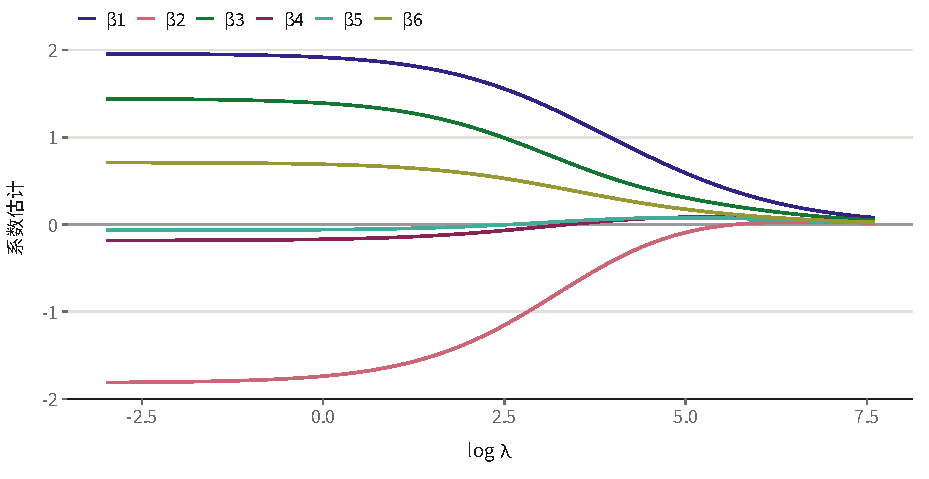
\includegraphics[width=\linewidth]{figures/ridge-path.pdf}
  \caption{Ridge coefficient paths. As $\lambda$ grows, every coefficient is pulled continuously towards zero.}
  \label{fig:path}
\end{figure}

\begin{table}[htbp]
  \centering
  \caption{Bias, variance and mean squared error for several values of $\lambda$}
  \label{tab:mse}
  \begin{tabular}{@{}rrrr@{}}
    \toprule
    $\lambda$ & $\norm{\Bias}_2^2$ & $\tr\Var$ & $\MSE$ \\
    \midrule
    0   & 0.000 & 0.449 & 0.449 \\
    1   & 0.008 & 0.424 & 0.432 \\
    2   & 0.029 & 0.402 & \textbf{0.430} \\
    5   & 0.148 & 0.345 & 0.493 \\
    20  & 1.110 & 0.195 & 1.305 \\
    100 & 4.030 & 0.048 & 4.078 \\
    \bottomrule
  \end{tabular}
\end{table}

\Cref{tab:mse} makes three points:
\begin{enumerate}
  \item the variance falls and the bias rises monotonically, as \cref{prop:bv} predicts;
  \item around $\lambda = 2$ the MSE is below that of least squares ($\lambda=0$);
  \item heavy shrinkage ($\lambda=100$) lets the bias dominate the risk.
\end{enumerate}

Computing the estimator takes one line of linear algebra:
\begin{lstlisting}[language=R]
ridge <- function(X, y, lambda) {
  p <- ncol(X)
  solve(crossprod(X) + lambda * diag(p), crossprod(X, y))  # normal equations
}
\end{lstlisting}

\section{Conclusion}

Ridge regression illustrates a recurring theme in statistics: \emph{unbiased is not the same as good}.
In practice $\lambda$ is chosen by cross-validation.

\printbibliography

\appendix
\section{An extra derivation}\label{app:extra}

For an orthogonal design $X^\top X = I_p$ the ridge estimator is a rescaled least-squares estimator:
\[
  \hat\beta_\lambda = \frac{1}{1+\lambda}\,\hat\beta^{\mathrm{OLS}},
  \qquad
  \MSE(\lambda) = \frac{p\,\sigma^2 + \lambda^2\norm{\beta}_2^2}{(1+\lambda)^2},
\]
which is minimised at $\lambda^\star = p\sigma^2/\norm{\beta}_2^2$.

\end{document}
